\chapter{Ergebnisse}
\label{ch:results}

In diesem Kapitel werden die Ergebnisse der in \autoref{subsec:experimente} beschriebenen Experimente vorgestellt.
Zunächst wird beschrieben wie die Modelle, die mit teils verschieden langer Clips trainiert wurden, einheitlich verglichen werden können.
Anschließend werden die Ergebnisse aller vier Phasen vorgestellt.
Die Evaluation endet mit einer Kategorisierung der Klassen in vier Schwierigkeitsgrade und einer Einschätzung welchen Grenzen das Training unterlag.

\section{Vergleichbarkeit der Ergbnisse}

In den folgenden Abschnitten werden die Rechenergebnisse verschiedener Modelle verglichen.
Die Modelle unterscheiden sich, wie schon in \autoref{tab:coverage} gezeigt, durch verschiedene Hyperparameter, die zu verschiedenen Werten der Clip-Dauer $\Delta$ führen.
Während des Trainings werden im Trainings- und Validierungsset Samples generiert, deren Länge $\Delta_\text{fit} = \frac{T}{\tau}$ von der Wahl der Hyperparameter $\gamma_\tau$ und $\delta_t$ abhängt.
Um vergleichbare Ergebnisse bei verschiedenen Hyperparametern zu gewährleisten, umfasst das Test-Set hingegen die immer gleichen Samples mit einer festen Clip-Dauer von $\Delta_\text{test}=6$, die sich an der maximalen Länge einer Spielaktion in \gls{sbod} (siehe \autoref{subsec:hyperparameter}) orientiert.

Die Wahl von $\gamma_\tau$ wird während der Evaluation in jedem Fall übernommen, da sie grundlegende Eigenschaften (wie die Geschwindigkeit) der Samples abbildet, auf die das vortrainierte Modell bereits zugeschnitten ist.
Die Test-Samples sind aber immer länger als die Trainings- und Validierungssamples mit $\Delta_\text{fit} < \Delta_\text{test}$.
Um diese Hürde zu überwinden, werden drei verschiedene Methoden verglichen, den Input des zu evaluierende Modells abzuändern:

\begin{description}
    \item[Avg-Consensus]
    Ein Test-Clip wird in mehrere zeitliche Crops segmentiert, die sich gleichmäßig über den gesamten Zeithorizont des Test-Clips verteilen und sich potentiell überschneiden.
    Die Crops werden einzeln inferiert und der endgültigen Score des Clips ergibt sich aus einer Aggregation (consensus function) über alle Crops.
    Als Aggregation wird in diesem Zusammenhang der Durchschnitt pro Klasse ermittelt.
    \item[Max-Consensus]
    Analoge Verarbeitung zu Avg-Consensus, wobei als Aggregation das Maximum pro Klasse berechnet wird.
    \item[Avg-Pooling]
    Der zeitliche Dimension $T$ des Test-Clip wird auf die nötige Anzahl erhöht, um die Test-Dauer zu erreichen.
    Alle trainierten Modelle verfügen über ein dynamischen Avg-\pool-Layer, das die Feature-Maps rechtzeitig wieder auf eine fixe Dimension für die hinteren \fc-Layer projeziert.
    Das Modell aggregiert die Informationen somit intern.
\end{description}

Während des Training werden stets 5-dimensionale Input-Batches $x_\text{fit} \in (B \times C \times T \times S^2)$ verwenden.
Bei der Evaluation wird nun eine weitere Dimension benötigt, um die verschiedenen Crops abzubilden mit $x_\text{test} \in (B \times E \times C \times T \times S^2)$.
Dabei stell $E$ die Anzahl der zeitlichen Crops dar.

Für ein vortrainiertes Modell mit maximaler Batchgröße $B_\text{fit}$ und Clip-Dauer $\Delta_\text{fit}$, lassen sich unter der Annahmen, dass das Produkt aller Dimension gleich bleibt, die maximalen Dimensionen für $x_\text{test}$ eindeutig ermitteln.
\autoref{eq:eval-dims-consensus} zeigt die Dimension für Avg- und Max-Consensus.

\begin{equation}
    \label{eq:eval-dims-consensus}
    \begin{split}
    E_\text{test}           & = \lceil  \frac{\Delta_\text{test}}{\Delta_\text{fit}}  \rceil \\
    T_\text{test}           & = T_{\text{fit}} \\
    B_\text{test}           & = \lfloor \frac{B_\text{fit}}{E_\text{test}} \rfloor
    \end{split}
\end{equation}

Alternativ werden im Falle des Avg-Pooling die Dimensionen wie in \autoref{eq:eval-dims-pool} gewählt.

\begin{equation}
    \label{eq:eval-dims-pool}
    \begin{split}
    E_\text{test}           & = 1 \\
    T_\text{test}           & = \lceil T_\text{fit} \frac{\Delta_\text{test}}{\Delta_\text{fit}} \rceil \\
    B_\text{test}           & = \lfloor \frac{T_\text{test} }{B_\text{fit} T_\text{fit}} \rfloor
    \end{split}
\end{equation}

\subsection{Initialisierungsphase und Vergleich temporärer Aggregation}
\label{subsec:initialisierungsphase}

In der ersten Phase der Experimente werden pro Modell vortrainierte (basierend auf Kinetics-400) und öffentlich zugängliche Gewichte in die Architektur geladen.
Das jeweils letzte \fc-Klassifikationslayer wird durch ein neues mit 32 Output-Klassen ausgetauscht und einzeln für einen Zyklus (siehe \autoref{subsec:trainingsschleife}) mit etwa $\Theta_\text{train} = 100$ Samples pro Klasse nachtrainiert.
\Dh alle übrigen Layer des Modells bleiben unverändert.
Erst in einer späteren Iteration werden alle Layer in einem zweiten Zyklus nachtrainiert.

Für alle der drei Backbones wird nach Abschluss des zweiten Zyklus evaluiert welches der oben genannten Aggregationsverfahren für die Test-Samples am besten geeignet ist.
Pro Backbone wird das Test-Set pro Verfahren getestet.
\autoref{fig:consensus} zeigt verschieden Metriken für jede der Aggregationen, sowie für das Validierungsset:

\begin{figure}[htbp!]
    \centering
    \begin{subfigure}{.5\textwidth}
        \centering
        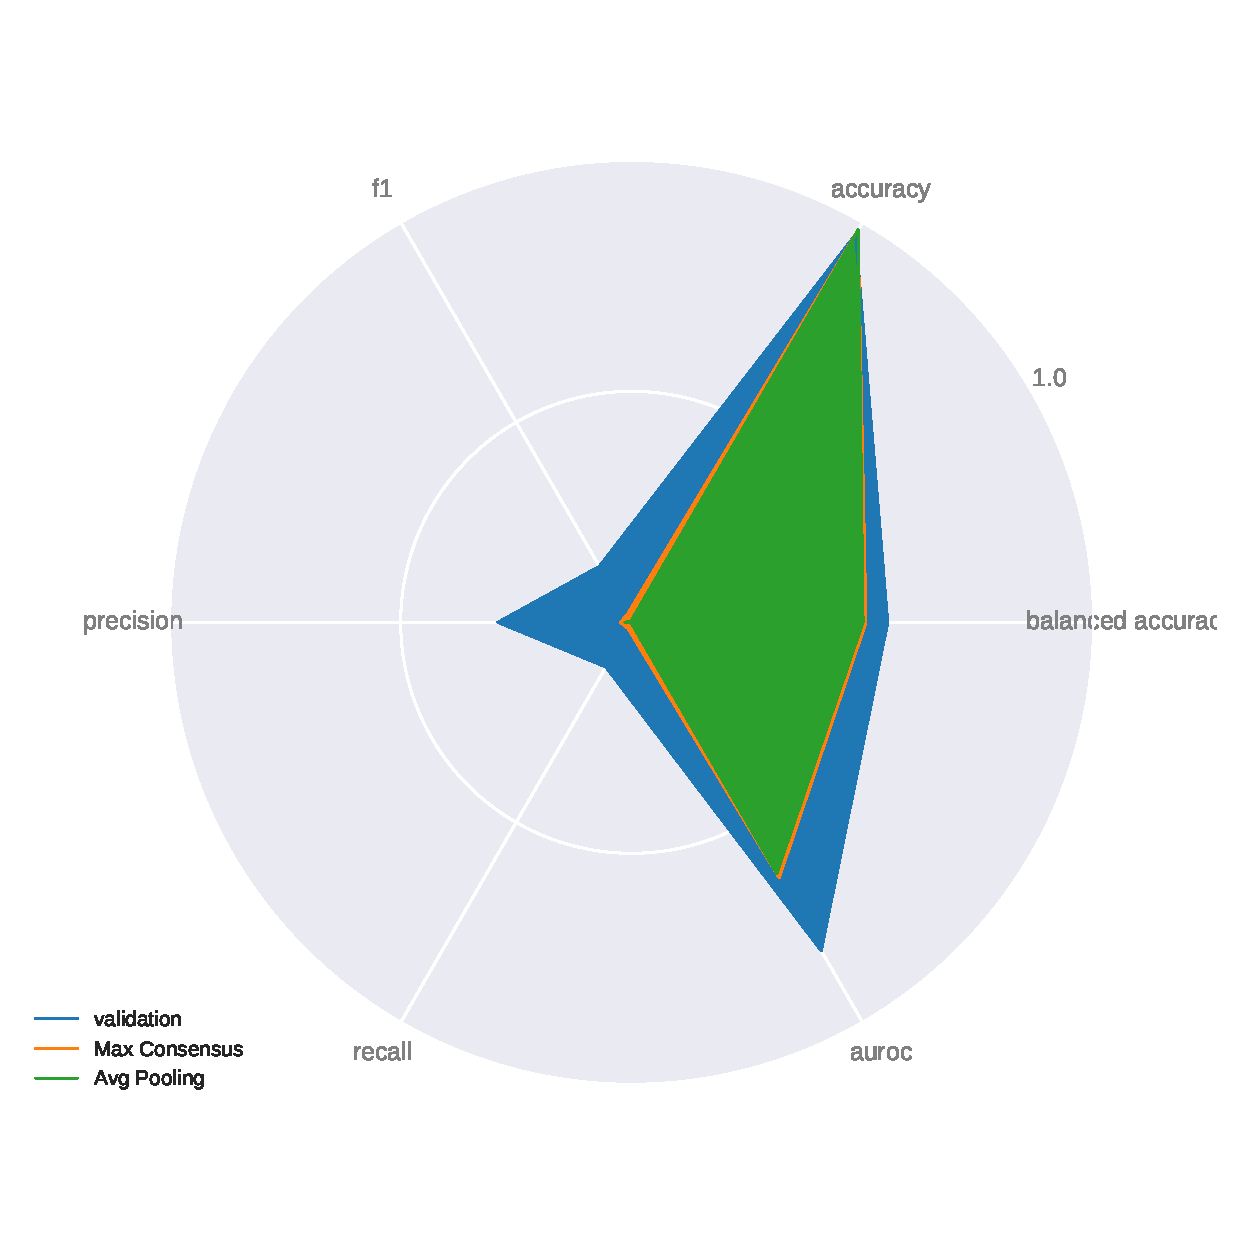
\includegraphics[width=0.8\textwidth, height=0.8\textwidth, keepaspectratio, interpolate]{img/07_consensus_radar.eps}
    \end{subfigure}%
    \begin{subfigure}{.5\textwidth}
        \centering
        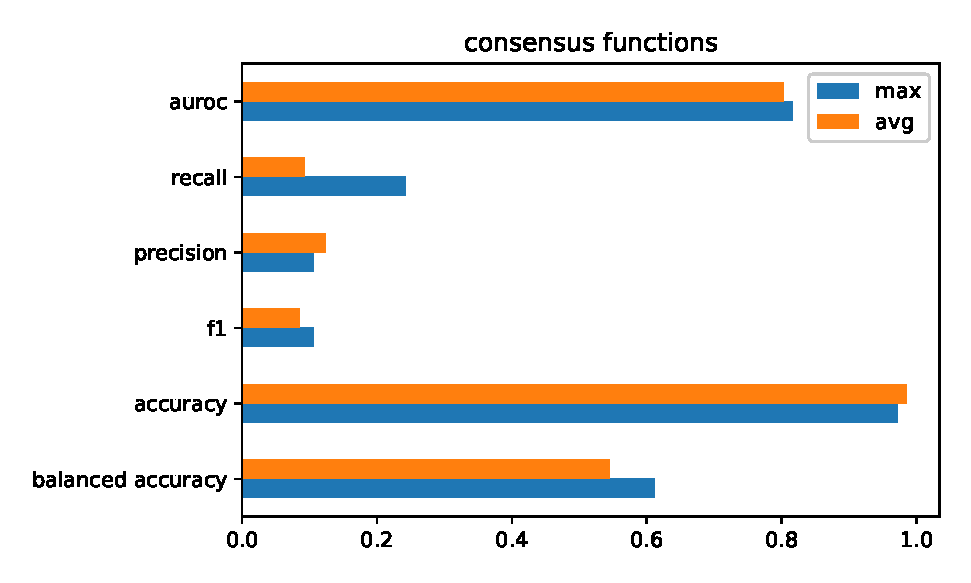
\includegraphics[width=0.8\textwidth, height=0.8\textwidth, keepaspectratio, interpolate]{img/07_consensus.eps}
    \end{subfigure}
    \caption{Vergleich von Max- und Avg-Aggregation am Test-Set (ir-CSN mit $\gamma_\tau = 2$) }
    \label{fig:consensus}
\end{figure}

Die Avg-Aggregation weist in allen Fällen eine knapp höhere Precision und Accuracy auf, während die Max-Aggregation einen deutlich höheren Recall, eine leicht höhere AUROC und Balanced Accuracy und in den meisten Fällen einen leicht höheren F1-Score.
Die Ergebnisse lassen sich zum Teil dadurch erklären, dass die Scores durch die Mittelung der Avg-Aggregation immer niedriger sind als die Scores in der Max-Aggregation, wodurch die Anzahl aller Positives insgesamt abnimmt.
Die Avg-Aggregation ist also deutlich sensibler gegenüber False Positives.

Dennoch wird die Avg-Aggregation als primäre Aggregation für den weiteren Verlauf festgelegt.
Zum einen, da die Metriken im Schnitt einen besseren Kompromiss darstellen.
Zum anderen, da sie die Realität logisch abbildet:
Enthält ein Clip von 10 Sekunden zwei Aktionen -- die eine Aktion ganz zu Beginn und die andere Aktion kurz vorm Ende, ist die erste Aktion nicht im letzten Chunk und die zweite Aktion nicht im ersten Chunk sichtbar.
Die Max-Aggregation kann derartige Zustände erkennen, da die Maxima sich auf die lokalen Stellen im Clip beziehen, während die Lokalität bei der Avg-Aggregation verwässert und ein hohes Maximum leicht durch weitere niedrige Scores überstimmt werden kann.

\section{Evaluation der Experimente}

Mit der zuvor festgelegten, einheitlichen Evaluationsmethode werden nun die Evaluationsergebnisse der einzelnen Experimente vorgestellt.
Diese bestehen zunächst aus einer Hyperparameter-Optimierung pro Modell, so wie einem semi-automatischen Verifikationsschritt, einem anschließenden Training auf einem teilweise bereinigten Datenset und einem weiteren Fine-Tuning.

\begin{tcolorbox}[title=Todo]
    \begin{itemize}
        \item jeweils epochen und $\gls{tld:Theta}_\text{train}$ nennen
        \item Grid-Search!! Wiederholen mit 100 Sampels, 5 Epochen, bessere Grid Auswahl
    \end{itemize}
\end{tcolorbox}

\subsubsection{Hyperparameter Optimierung}

Spielaktionen können unter Berufung auf \gls{sbod} zwischen bis zu 6 Sekunden dauern.
Die vortrainierten Modelle bilden in ihrer ursprünglichen Form jedoch maximal 2.56 Sekunden ab.
Im Zuge der zweiten Experimentphase werden verschiedene Hyperparameter mithilfe einer gierigen Grid-Suche getestet.

Alle Modelle nutzen eine dynamisches Avg-\pool-Layer zwischen dem letzten \conv- und dem ersten \fc-Layer, das die Verarbeitung von Tensoren variabler Länge $T$ zulässt.
Um eine geeignete Methode zu finden, wird der Einfluss von Avg-Pooling und von Subsampling auf den jeweils gleichen Daten pro Modell verglichen.

Die Grid-Suche betrachtet Punkte für verschiedene $\gamma_t$ und $\gamma_\tau$.
Beginnend mit einer Startkonfiguration (Baseline-Modell), werden iterativ beide Parameter einzeln erhöht, sodass sich die in beiden Fällen die gleiche Clip-Dauer ergibt.
Die Konfigurationen werden verglichen und die erfolgreichere wird wieder zum Startpunkt für die nächste Iteration.
Die Suche endet sobald, es keine Verbesserungen mehr gibt oder ein Training aufgrund von Hardwarebeschränkungen nicht mehr möglich ist.
Mit den genannten Einschränkung ist die Suche deutlich schneller, aber auch unvollständiger als eine gewöhnliche Grid-Suche.

\begin{figure}
    \centering
    \csvreader[no head,tabular=|l|r|r|r|r||r|r|r|,
    table head=\hline,late after line=\\\hline]{tbl/pre-eval.csv}
    {1=\model,2=\s,3=\t,4=\sr,5=\d,6=\result,7=\ihatelatex,8=\reallyshittylatex}
    {\model & \s & \t & \sr & \d & \result & \ihatelatex & \reallyshittylatex}
    \caption{Ergebnisse zur Hyperparameter-Optimierung}
    \label{tab:pre}
\end{figure}

\begin{figure}
    \centering
    \begin{subfigure}{.33\textwidth}
        \centering
        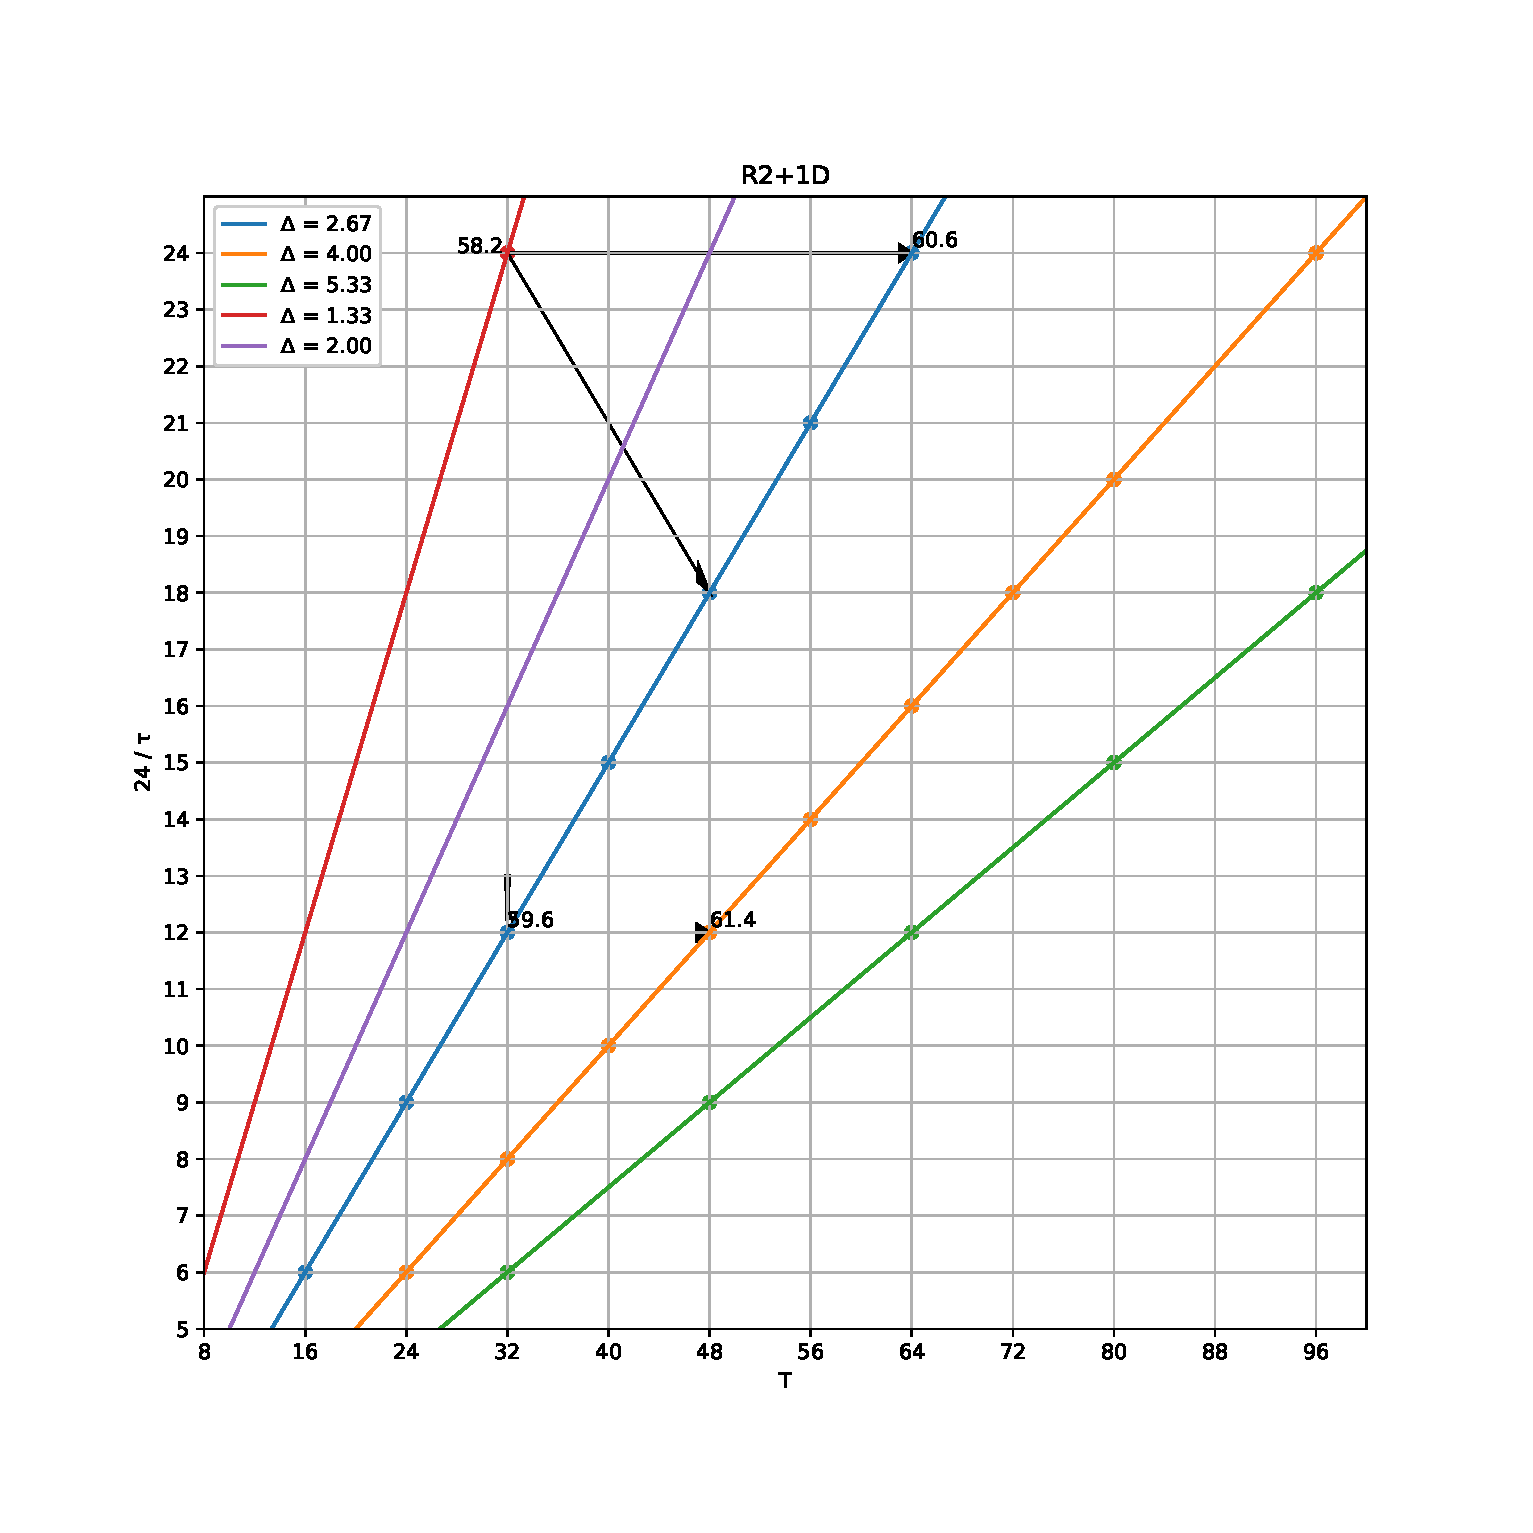
\includegraphics[width=0.99\textwidth, height=0.8\textwidth, keepaspectratio, interpolate]{img/07_grid_r2plus1d.eps}
    \end{subfigure}%
    \begin{subfigure}{.33\textwidth}
        \centering
        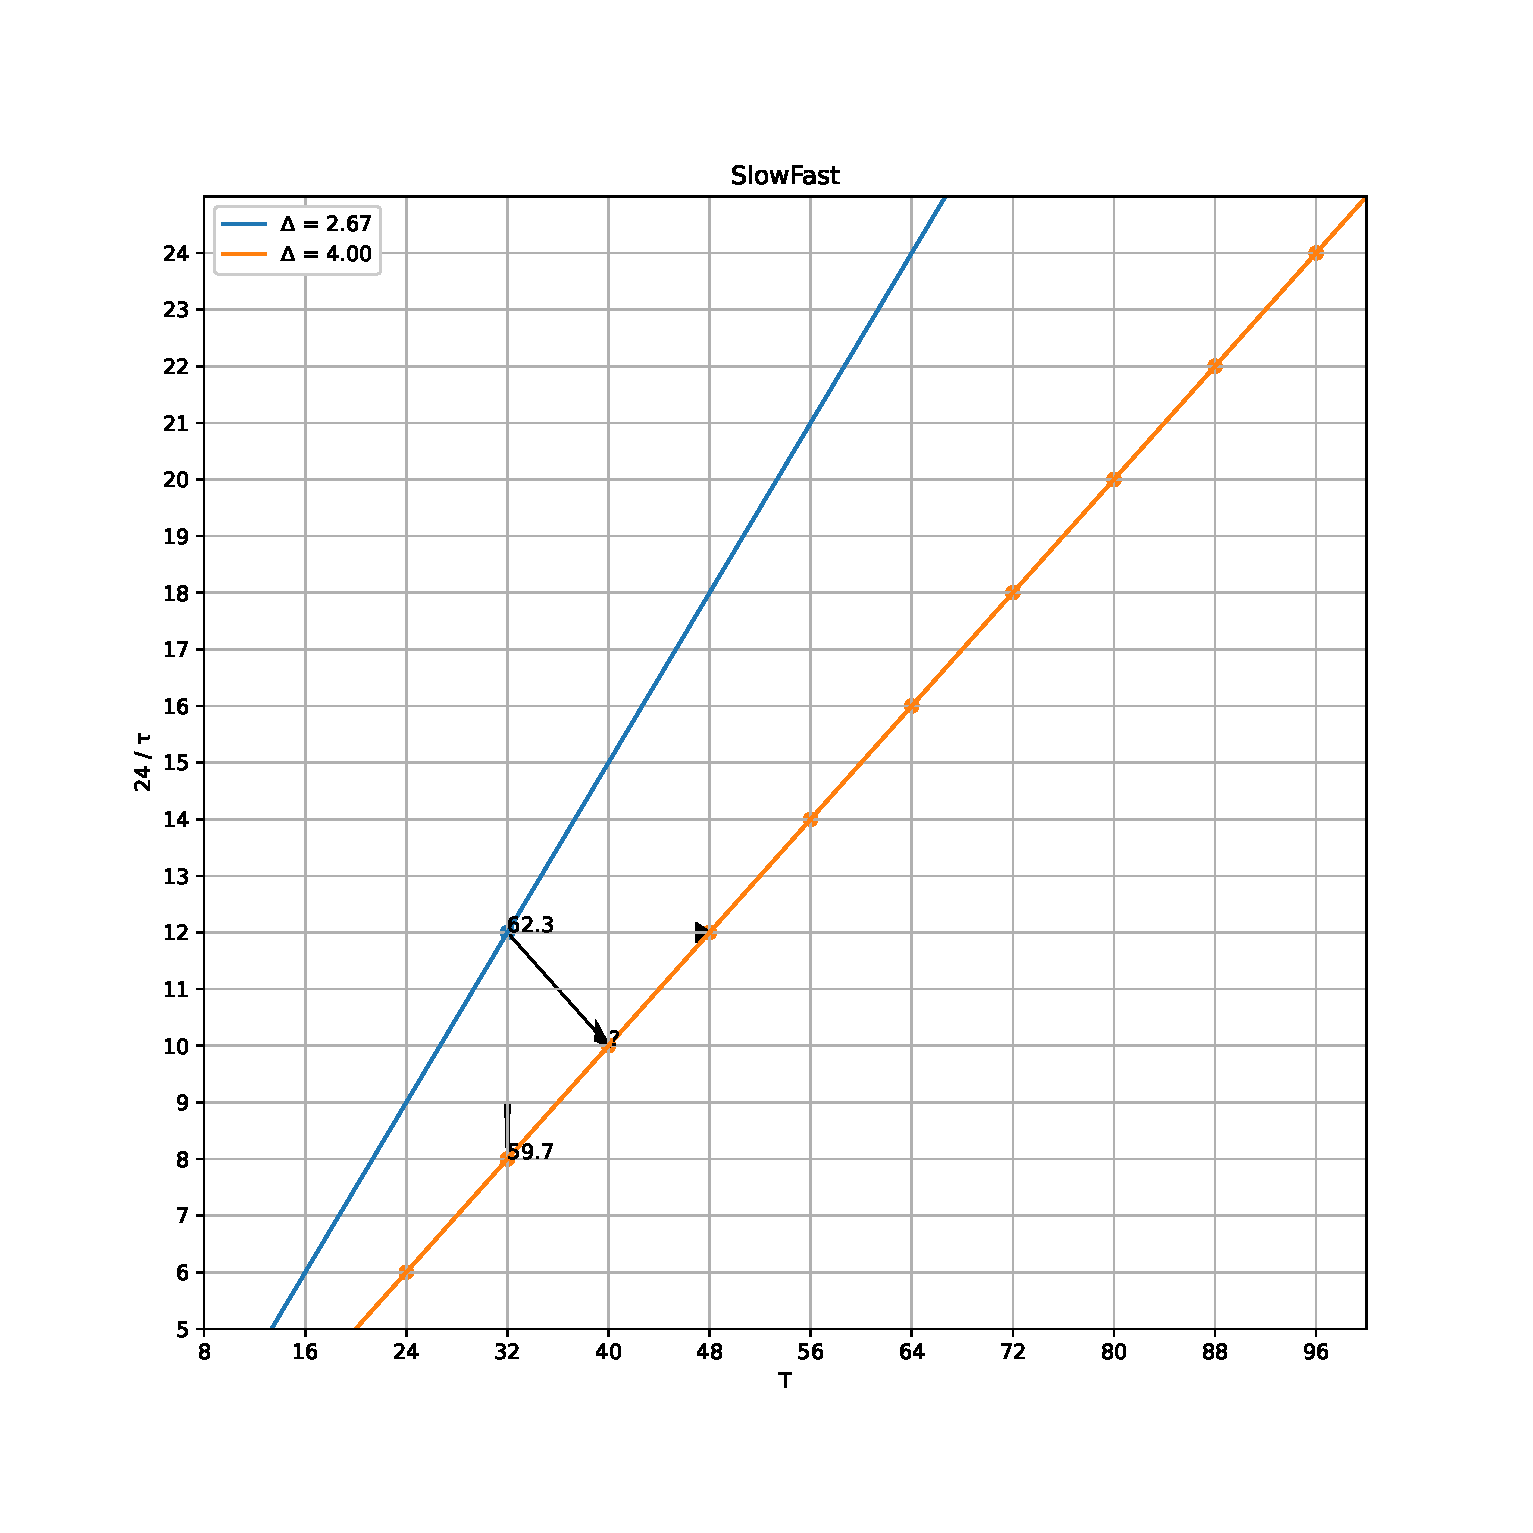
\includegraphics[width=0.99\textwidth, height=0.8\textwidth, keepaspectratio, interpolate]{img/07_grid_slowfast.eps}
    \end{subfigure}
    \begin{subfigure}{.33\textwidth}
        \centering
        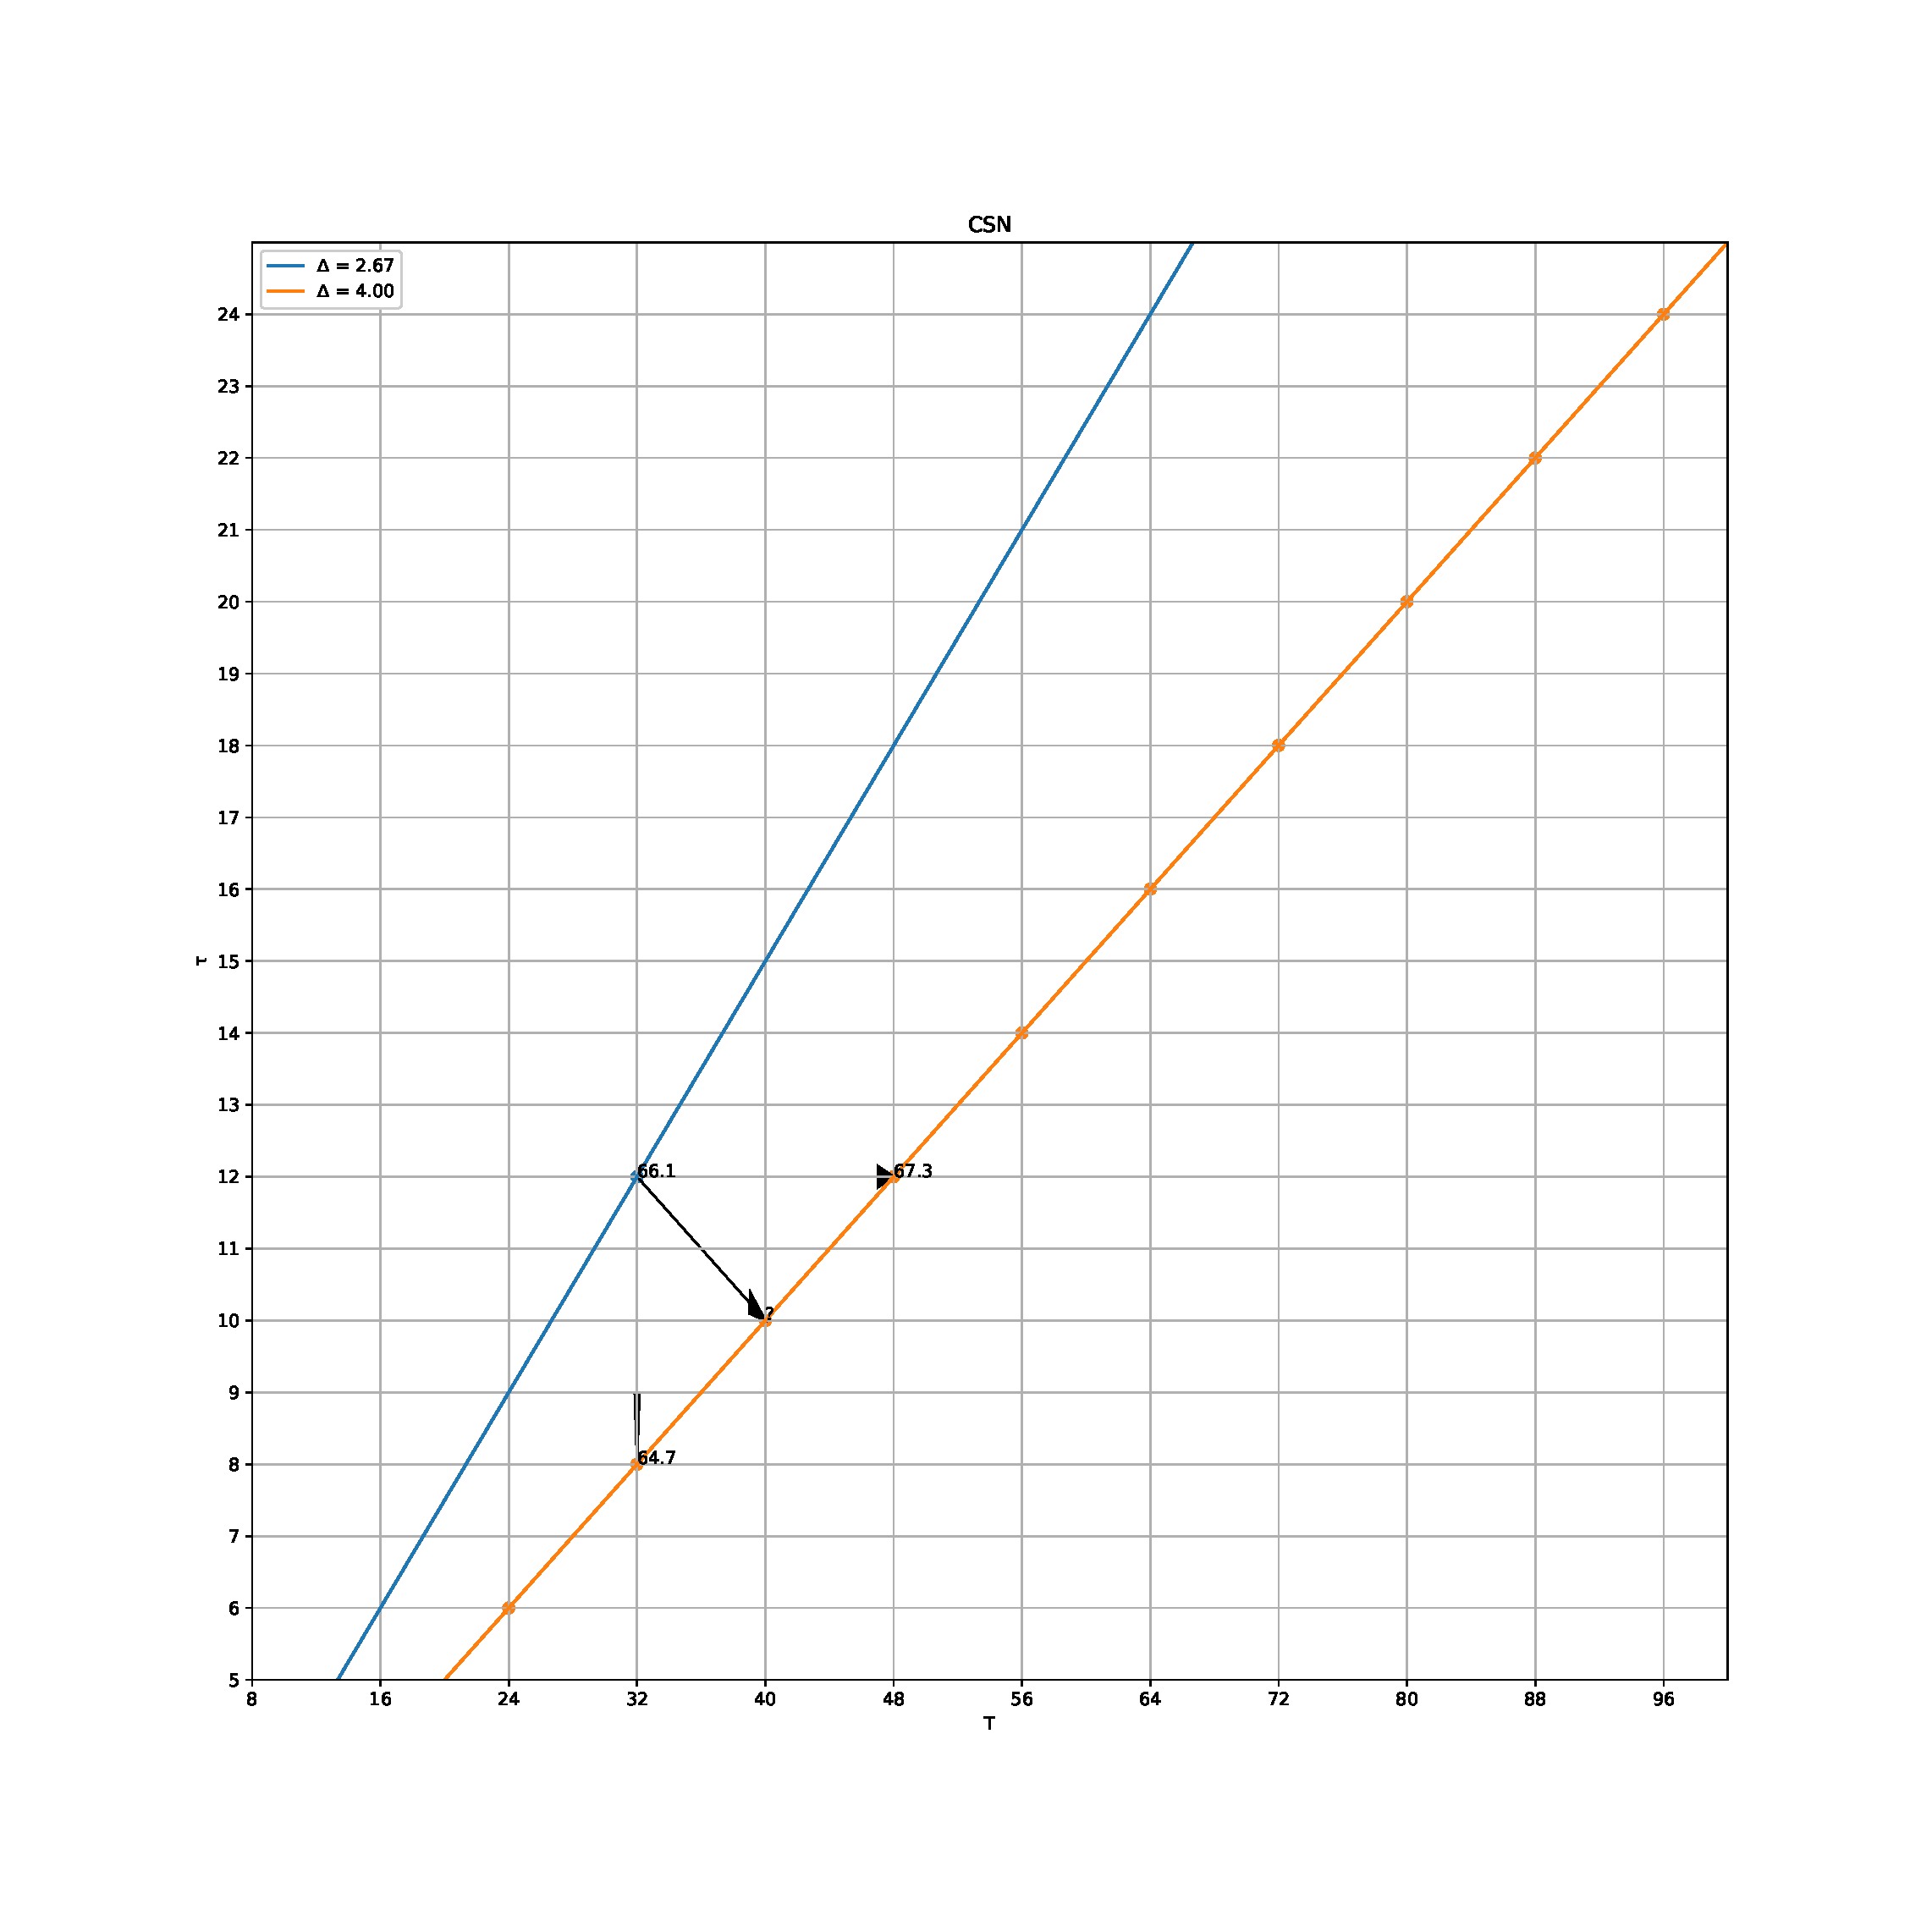
\includegraphics[width=0.99\textwidth, height=0.8\textwidth, keepaspectratio, interpolate]{img/07_grid_csn.eps}
    \end{subfigure}
    \caption{Grid-Suche für optimale Hyperparameter}
    \label{fig:exp-hparams}
\end{figure}

\autoref{tab:pre} und \autoref{fig:exp-hparams} zeigt die Ergebnisse, indem pro Modell ausgehend von das Baseline-Konfiguration die Clip-Dauer erhöht wird.
Die Experimente in \autoref{tab:pre} wurden dazu mit $\gls{tld:Theta}_\text{train} = 100$ Samples pro Klasse (inklusive 100 Background-Samples) zu je 5 Epochen durchgeführt.

\subsubsection{Verifikation}

\begin{tcolorbox}[title=Todo]
    \begin{itemize}
        \item protokoll: Abbruchbedingung sinnvoll?
        \item beispiele im Anhang?,
        \item häufige fehler (Datenfehler, Klassifikationsfehler),
        \item basis: beste ep
        \item Anzahl = 25 ?
    \end{itemize}
\end{tcolorbox}


In der dritten Phase werden diejenigen Samples, die den größen Loss innerhalb eines Trainings vorweisen, genauer analysiert.
Grundlage ist eine Analyse der Experimente aus Phase 2.
In Zuge der Analyse werden zum einen Datenfehler (wie in \autoref{sec:nachgang} beschrieben) behoben.
Zusätzlich werden manuell Informationen über die $25$ größten Fehler (abhängig vom Loss im Fehlerreport) innerhalb eines Experiments erhoben.

Die Analyse folgt einem definiertem Protokoll:
Sind alle Experimente einer Phase abgeschlossen, wird zunächst eine neue Transaktionsdatei erstellt.
Für jedes der genannten Durchläufe (der jeweiligen Phase) wird das Relabel-Tool mit den persistierten Score- und Loss-Werte des je letzten Epoche initialisiert.
Das Relabel-Tool erhält ebenfalls Zugriff auf die Datenbankinstanz, die sich aus der persistierten JSON-Datenbank und den in dieser Phase bereits durchgeführten Transaktionen zusammensetzt.
So kann das Relabel-Tool \ua erkennen, das der selbe Fehler schon in einem vorherigen Experiment behoben wurde.

Die Samples werden absteigend nach Loss-Wert sortiert und dem Nutzer iterativ präsentiert.
Der Nutzer kann das Sample als Datenfehler in Form einer Transaktion beheben oder als Klassifikationsfehler markieren.
Als Klassifikationsfehler markierte Samples werden automatisch geloggt und im Cloud-Speicher abgelegt.
Die Analyse kann abgebrochen werden, sobald mindestens $25$ Klassifikationsfehler erfasst wurden.

\subsubsection{Fine-Tuning und Benchmark}

\begin{tcolorbox}[title=Todo]
    \begin{itemize}
        \item Zudem werden der Einfluss verschiedener Auflösungen verglichen.
        \item Label Smooting
        \item anpassung pro modell: reaktiv auf Phänome, wie Overfitting, Optimierung pro Modell (Anzahl Epochen, Weight Decay, Tiefere Modelle)?
    \end{itemize}
\end{tcolorbox}

In der vierten Phase werden die besten Modelle aus Phase 2 mit bis zu $\gls{tld:Theta}_\text{train} = 250$ Samples pro Klasse auf Grundlage der verifizierten Datenbank aus Phase 3 nachtrainiert.
Anschließend wird reaktiv auf die Ergebnisse des Trainings reagiert.
\autoref{tab:exp4} zeigt die Ergebnisse.

\begin{figure}
    \centering
    \csvreader[no head,tabular=|l||r|r|r||r|r|r|,
    table head=\hline,late after line=\\\hline]{tbl/exp_phase_4.csv}
    {1=\model,2=\s,3=\t,4=\sr,5=\d,6=\result,7=\ihatelatex}
    {\model & \s & \t & \sr & \d & \result & \ihatelatex}
    \caption{Ergebnisse zur Fine-Tuning}
    \label{tab:exp4}
\end{figure}


\section{Kategorisierung der Aktionsklassen}

\begin{tcolorbox}[title=Todo]
    \begin{itemize}
        \item Abweichung pro Metrik erheben: Klasse zu macro -> Durchschnitt
        \item Idee: pca und clustering in vier gruppen
        \item Vergleich der Evaluation auf subsets (SOCC-HAR-8, -16, -24, -32)
        \item Optional: SOCC-HAR-NET, SOCC-HAR-DB Klassen
    \end{itemize}
\end{tcolorbox}

Da ein Großteil der in \autoref{subsec:metriken} vorgestellten Metriken pro Klasse erhoben werden, kann eine genauere Analyse über die Komplexität zur Klassifizierung einer einzelnen Klasse gemacht werden.
Wie einfach oder schwer eine Klasse zu lernen ist, soll pro Modell und Modell-übergreifend veranschaulicht werden.

\subsection*{Vergleich mit Klassen aus SoccerNet, SoccerDB}

\section{Grenzen und Hypothesen}

\begin{tcolorbox}[title=Todo]
    Desweiteren sind bis auf AUROC alle Metriken durch einen Score-Grenzwert definiert, der angibt ab welcher Sicherheit ein Label für einen Score-Wert übernommen wird.
    Initial liegt der Grenzwert bei 50 \%.
    Wenn der Label-Score eines Samples über 50 \% liegt, wird es \ua mit diesem Label klassifiziert.
    Es kann entweder ein globaler Score-Grenzwert für alle Labels oder individuelle Grenzwerte pro Label gesetzt werden.
    Um einen geeigneten globalen Score-Wert zu finden werden vorab verschiedene Grenzwerte (an Balanced Accuracy) ausprobiert, der für alle weiteren Metriken verwendet wird.
\end{tcolorbox}

% \section{Grenzen und Hypothesen}

%\section{Anwendung der Modelle auf SoccerNet-500}
%\label{sec:anwendung-der-modelle-auf-soccernet-500}

%Im ersten Durchgang werden alle Modelle mit Daten aus SoccerNet-500 trainiert.

%Die Daten werden wie im Original-Paper nach Spiel aufgeteilt im Verhältnis (3:2:1).
%Für jede Annotation wird ein Eintrag im Datenframe erstellt, sowie für jede Spielminute, in der keine der drei definierten Aktionen stattfindet.
%Während in SoccerNet das ganze Videomaterial von einer Minute komprimiert wurde, werden in diesem Aufbau nur Tensoren von 5 Sekunden als Input genutzt.
%Für die Spielminuten ohne Annotation wird eine Hintergrund-Aktion in der 30. Sekunde der Spielminute erstellt, sodass es zu keiner potenziellen Überschneidung kommen kann.

%Aus dem Datenframe werden anschließend H5-Datensets mit je 400 (50 und 100) Trainings- (Validierungs- und Test-) samples pro Klasse gespeichert.

%\subsection{Ergebnisse}

%<<tab:soccernet>> zeigt die Ergebnisse des ersten Durchlaufs.

%\begin{figure}
%    \centering
%    \csvautotabular{tbl/s.csv}
%    \caption[]{Vergleich SoccerNet Benchmark}
%    \label{tab:soccernet}
%\end{figure}

%In alle Modellen wurden nur die hinteren \fc-, sowie Teile des letzten \res-Layers trainiert, sodass die Zahl der trainierbaren Parameter etwa gleich sind pro Modell.
%Weitere Layer wurden bewusst nicht trainiert, um ein Overfitting zu vermeiden.
%Für alle Modelle gilt, dass sie ab einer gewissen Epoche overfitten, was auf zu wenig Samples zurückzuführen ist.
%Insbesondere ip-CSN ist schwer zu trainieren, da es aufgrund der hohen Auflösung viel Speicher einnimmt und somit nur eine kleine Batchgröße ermöglicht.
%Im Gegenseatz zu Slowfast, das die selbe Auflösung verarbeitet, werden in ip-CSN alle Frames des Tensors verarbeitet (in Slowfast nur jeder zweite).
